\section{Evaluation}
\label{sec:eval}

We evaluate \textsc{StratQ} across six workload families and eleven database/modern operator adaptations plus an independent grouped hypergeometric CS to answer five questions:
(Q1) Does \textsc{StratQ} achieve real end-to-end latency speedups and reliable decision certification on expensive GPU neural predicates?
(Q2) How does \textsc{StratQ} compare against modern 2025--2026 statistical and database comparators (\texttt{Spertus-WoR}, \texttt{CELEUS-FixedProxy}, \texttt{Calibrated-FixedProxy}, \texttt{BARGAIN-Global}, \texttt{PilotDB-Asymp})?
(Q3) Does Safe-LOO range--variance gating deliver strong savings on accurate proxies without degrading under noisy or weak proxies?
(Q4) How do \textsc{StratQ}'s guarantees and cost behave across classical grouped AQP baselines, decision boundaries, and high group counts under Zipf skew?
(Q5) How do DuckDB+Arrow profiling, query reuse, and isolated memory footprint scale to 10 million rows?

\subsection{Experimental Setup and Comparators}
\label{sec:eval-setup}

\paragraph{Environment}
All experiments run on Windows 11 with Python 3.12, DuckDB 2.0.1, PyArrow 21.0, PyTorch 2.8.0 (CUDA 12.9), and an NVIDIA GeForce RTX 4060 Laptop GPU (8\,GiB VRAM).
Unless noted otherwise, every \textsc{StratQ} arm enforces nominal $90\%$ joint simultaneous coverage ($\delta = 0.1$) with \texttt{gating\_mode="safe\_loo"} and \texttt{safe\_rounding=True}; external adaptations use their documented interval implementations.

\paragraph{Six workload families}
(1)~\textbf{Yelp-DistilBERT-SST2} (live GPU text): 20,000 Yelp test reviews partitioned into $G=5$ star-rating groups ($N_g \in [3{,}791, 4{,}108]$); reference predicate is DistilBERT-SST2 on GPU (batch 64/128/256), and proxy is a CPU TF-IDF + Logistic Regression trained on a disjoint 18,000-row prefix.
(2)~\textbf{CIFAR10-ResNet34-GPU} (live GPU vision): 10,000 CIFAR-10 test images across $G=10$ classes ($N_g = 1{,}000$ each); reference predicate is an ImageNet-pretrained ResNet34 fine-tuned and evaluated on GPU at standard $224\times 224$ resolution to detect animal classes, and proxy is a CPU logistic model on $4\times 4$ RGB averages plus channel standard deviations (51 features).
(3)~\textbf{Fashion-MNIST} (live CPU vision): 10,000 official test images in $G=5$ brightness bins; RBF-SVM reference vs.\ pooled-pixel logistic proxy ($\epsilon_g = 0.04 N_g$).
(4)~\textbf{SMS Spam} (live CPU text): 2,271 deduplicated held-out messages across $G=5$ length groups; character-feature $k$-NN reference vs.\ word-feature logistic proxy ($\epsilon_g = 0.06 N_g$).
(5)~\textbf{UCI Adult} (tabular replay): 16,281 official test rows across $G=9$ workclass groups ($\epsilon_g = 0.04 N_g$), using education-rate proxy plus \texttt{age} and \texttt{hours} covariates.
(6)~\textbf{Synthetic Parquet Scale \& Stress}: 12K-row proxy-quality sweep ($G=8$), 100K-row Zipf skew sweep ($G \in \{5,10,20,50,100\}$, $\alpha_{\text{zipf}} \in \{0.0, 0.8, 1.2\}$), and 100K--10M-row Parquet snapshots ($G=20$).

\paragraph{Eleven operator comparators}
We separate \emph{modern 2025--2026 operator adaptations} from \emph{classical AQP operators}; none is claimed as a full system replica, and all contract differences are audited in our artifact documentation.
Modern comparators:
\textbf{Spertus-WoR} (adapted from~\cite{spertus2026sequential}: uniform within-group WoR, max-slack routing, zero predictor, Bonferroni risk);
\textbf{CELEUS-FixedProxy} (adapted from~\cite{zhou2026celeus}: fixed surrogate-completed IPW signal and hedged-capital e-process inversion across groups);
\textbf{Calibrated-FixedProxy} (independent control, not a named system replica: one Ridge predictor fitted on the same pilot prefix and frozen permanently while sharing \textsc{StratQ}'s permutations, routing, and safe CS);
\textbf{BARGAIN-Global} (adapted from~\cite{zeighami2026bargain}: single global anytime count target with proportional plug-in group estimates); and
\textbf{PilotDB-Asymp} (adapted from~\cite{zhu2025pilotdb}: two-stage CLT simultaneous normal intervals with finite-population correction, evaluated under an optional-stopping diagnostic to expose asymptotic failure).
Classical comparators on Adult (at matched budgets $B \in \{2{,}048, 4{,}096, 8{,}192\}$): \textbf{ABae-inspired} two-stage proxy strata~\cite{kang2021abae}, \textbf{BlazeIt-inspired} fixed-look control-variate EB~\cite{kang2019blazeit}, \textbf{Congressional Senate} equal-quota hypergeometric~\cite{acharya2000congress}, \textbf{Online Aggregation} unindexed Hoeffding scan~\cite{hellerstein1997online}, \textbf{LWS} Des Raj normal~\cite{walenz2019lws}, and \textbf{VerdictDB} variational subsampling~\cite{park2018verdict}. An independent grouped hypergeometric CS~\cite{wor2020} is reported separately, yielding twelve non-\textsc{StratQ} methods in total.

\subsection{Live GPU Workloads and Modern Comparators}
\label{sec:eval-gpu}

\begin{figure*}[t]
\centering
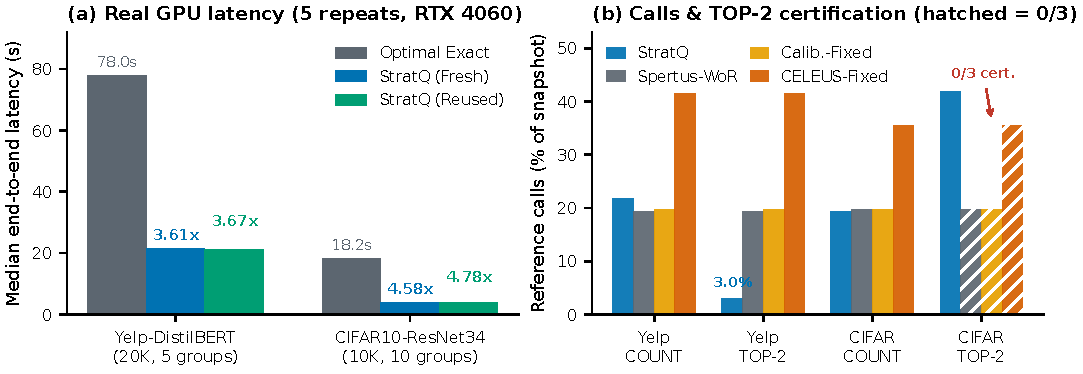
\includegraphics[width=\textwidth]{fig2_gpu_workloads.pdf}
\Description{Two-panel figure comparing StratQ against optimal exact GPU inference and modern operator baselines on Yelp-DistilBERT-SST2 and CIFAR10-ResNet34-224 after proxy scoring, showing 3.61x to 4.78x ratio-of-medians speedups and certified TOP-2 call efficiency under dedicated versus post-hoc COUNT-derived routing.}
\caption{Live GPU evaluation on RTX 4060 after proxy scoring. (a) Median grouped \texttt{COUNT} latency over 5 repeats vs.\ the fastest tested exact GPU batch size (batch 128 on Yelp, 64 on CIFAR-10); fresh/reused profiles win at modeled $Q=1$ under this setup boundary. (b) Reference calls (\% of snapshot) for \texttt{COUNT} and \texttt{TOP-2}; hatched bars indicate $0/3$ certification on CIFAR-10's 2-image rank gap under the post-hoc \texttt{COUNT}-derived protocol.}
\label{fig:gpu}
\end{figure*}

\begin{table*}[t]
\centering
\footnotesize
\setlength{\tabcolsep}{4pt}
\caption{Live GPU expensive-predicate evaluation (3 seeds per query, $\delta=0.1$, $\epsilon_g=0.04 N_g$). Calls are means; sample SD and ranges are reported in the text. \texttt{COUNT Wall} excludes profile construction. \texttt{BARGAIN-Global} satisfies only a global target ($0/3$ all-group coverage). For non-\textsc{StratQ} baselines, \texttt{HAVING}/\texttt{TOP-2} decisions are derived from their \texttt{COUNT} intervals; \textsc{StratQ} runs dedicated boundary-focused routing under the same joint event.}
\label{tab:gpu-main}
\begin{tabular}{@{}llrrrrrr@{}}
\toprule
Workload & Method & \texttt{COUNT} Calls (\%) & Cov. & \texttt{COUNT} Wall (s) & \texttt{HAVING} Calls (Res./Corr.) & \texttt{TOP-2} Calls (Cert./Corr.) & Speedup vs.\ Exact \\
\midrule
\multirow{5}{*}{\shortstack[l]{Yelp-DistilBERT\\(20K, $G=5$,\\Exact 77.99\,s)}}
& \textbf{\textsc{StratQ} (\texttt{safe\_loo})} & 4,349 (21.7\%) & \textbf{3/3} & 17.47 & 4,390 (\textbf{3/3} / \textbf{3/3}) & \textbf{595 (3.0\%)} (\textbf{3/3} / \textbf{3/3}) & \textbf{3.61$\times$ / 3.67$\times$} \\
& Spertus-WoR~\cite{spertus2026sequential} & \textbf{3,859} (19.3\%) & 3/3 & 15.95 & 3,859 (0/3 / 3/3) & 3,859 (19.3\%) (3/3 / 3/3) & --- \\
& Calibrated-FixedProxy & 3,944 (19.7\%) & 3/3 & 15.43 & 3,944 (0/3 / 3/3) & 3,944 (19.7\%) (3/3 / 3/3) & --- \\
& CELEUS-FixedProxy~\cite{zhou2026celeus} & 8,296 (41.5\%) & 3/3 & 33.56 & 8,296 (0/3 / 3/3) & 8,296 (41.5\%) (3/3 / 3/3) & --- \\
& BARGAIN-Global~\cite{zeighami2026bargain} & 819 (4.1\%) & \textbf{0/3} & 3.13 & 819 (0/3 / \textbf{0/3}) & 819 (4.1\%) (0/3 / \textbf{0/3}) & --- \\
\midrule
\multirow{5}{*}{\shortstack[l]{CIFAR10-ResNet34\\(10K, $G=10$,\\Exact 18.22\,s)}}
& \textbf{\textsc{StratQ} (\texttt{safe\_loo})} & \textbf{1,936 (19.4\%)} & \textbf{3/3} & \textbf{2.82} & 4,421 (\textbf{3/3} / \textbf{3/3}) & \textbf{4,187 (41.9\%)} (\textbf{3/3} / \textbf{3/3}) & \textbf{4.58$\times$ / 4.78$\times$} \\
& Spertus-WoR~\cite{spertus2026sequential} & 1,979 (19.8\%) & 3/3 & 2.85 & 1,979 (0/3 / 3/3) & 1,979 (19.8\%) (\textbf{0/3} / \textbf{0/3}) & --- \\
& Calibrated-FixedProxy & 1,979 (19.8\%) & 3/3 & 2.97 & 1,979 (0/3 / 3/3) & 1,979 (19.8\%) (\textbf{0/3} / \textbf{0/3}) & --- \\
& CELEUS-FixedProxy~\cite{zhou2026celeus} & 3,557 (35.6\%) & 3/3 & 5.07 & 3,557 (0/3 / 3/3) & 3,557 (35.6\%) (\textbf{0/3} / 1/3) & --- \\
& BARGAIN-Global~\cite{zeighami2026bargain} & 733 (7.3\%) & \textbf{0/3} & 1.13 & 733 (3/3 / \textbf{0/3}) & 733 (7.3\%) (\textbf{0/3} / \textbf{0/3}) & --- \\
\bottomrule
\end{tabular}
\end{table*}

Figure~\ref{fig:gpu} and Table~\ref{tab:gpu-main} summarize both live GPU workloads (peak VRAM 1.29\,GiB on Yelp and 2.03\,GiB on CIFAR-10).

\paragraph{Descriptive variability (three seeds).}
\texttt{COUNT} calls are mean $\pm$ sample SD [range]: on Yelp, \textsc{StratQ} $4{,}349\pm74$ [4{,}264, 4{,}392] vs.\ Spertus-WoR $3{,}859\pm98$ [3{,}752, 3{,}944]; on CIFAR-10, $1{,}936\pm128$ [1{,}808, 2{,}064] vs.\ $1{,}979\pm133$ [1{,}872, 2{,}128]. Decision-call SD/ranges are in the artifact. These fixed-snapshot results are descriptive, not significance tests or population coverage estimates.

\paragraph{Query-level GPU latency after proxy scoring.}
Five repeats (seeds 5000--5004; tolerances 3/4/5/3/4\%) give median [range] latency: Yelp 77.99 [65.46, 87.78]\,s exact, 21.62 [14.22, 27.32]\,s fresh-profile, and 21.24 [14.73, 28.19]\,s reused; CIFAR-10 18.22 [17.74, 18.58]\,s, 3.98 [3.37, 5.30]\,s, and 3.81 [3.42, 5.23]\,s. Ratio-of-medians speedups are \textbf{3.61$\times$ fresh / 3.67$\times$ reused} and \textbf{4.58$\times$ / 4.78$\times$}. Proxy scores are precomputed and the GPU model/OS cache is warm; ``fresh'' only rebuilds the \texttt{TableProfile}, and the frozen run shared the $\psi$ cache. Fitting, loading, and proxy scanning are excluded. Adding Yelp's 3.97\,s scan gives 3.05$\times$/3.09$\times$; adding 6.75\,s training as first-query setup gives 2.41$\times$ fresh. CIFAR's scan time was not recorded.

\paragraph{Decision certification vs.\ modern comparators}
The sharpest separation emerges on SQL decision queries:
\begin{itemize}
  \item \textbf{Yelp \texttt{TOP-2} and \texttt{HAVING}:} Groups 4 and 5 (3,398 and 3,406 positives) separate from group 3 (2,178). With dedicated boundary routing, \textsc{StratQ} certifies exact \texttt{TOP-2} membership in \textbf{594.7 reference calls ($3.0\%$ of rows)} with $3/3$ accuracy---$6.5\times$ fewer than the Spertus-WoR adaptation (3,858.7), $6.6\times$ fewer than Calibrated-FixedProxy (3,944.0), and $13.9\times$ fewer than CELEUS-FixedProxy (8,296.0). On \texttt{HAVING} ($\tau=2{,}178$, exactly group 3's true count), it resolves all groups $3/3$ correctly, whereas the post-hoc \texttt{COUNT}-derived protocol leaves the boundary group unresolved ($0/3$ fully resolved). The global-count surrogate misclassifies groups ($0/3$ correct); this does not evaluate BARGAIN's original global guarantee.
  \item \textbf{CIFAR-10 \texttt{COUNT} and extreme 2-image \texttt{TOP-2}:} On \texttt{COUNT}, \textsc{StratQ} uses 1,936.0 calls (2.82\,s), vs.\ 1,978.7 for Spertus-WoR and Calibrated-FixedProxy and 3,557.3 for CELEUS-FixedProxy. On \texttt{HAVING} ($\tau=979$), dedicated routing resolves all groups $3/3$, while the post-hoc protocol fully resolves $0/3$. On \texttt{TOP-2}, the top four animal classes have true counts $(999, 996, 994, 993)$---only \textbf{2 images} between ranks 2 and 3. \textsc{StratQ} certifies the exact set in $3/3$ runs (4,186.7 calls, $41.9\%$ of rows). Under their respective \texttt{COUNT} stopping budgets, the post-hoc comparators certify $0/3$ and return wrong point rankings ($0/3$ or $1/3$); this does not establish how equal-budget decision-aware baseline routing would perform.
\end{itemize}

\paragraph{Honest boundary observation on Yelp \texttt{COUNT}.}
\textsc{StratQ} uses $4{,}349\pm74$ calls vs.\ $3{,}859\pm98$ for Spertus-WoR and $3{,}944\pm64$ for Calibrated-FixedProxy (mean$\pm$SD, $n=3$). A 202-decision trace selects a proxy in 112 batches, falls back for no cost improvement in 75, and for insufficient history in 15. Selected candidates reduce mean LOO variance by 12.9\%, but maximum prediction span is $8.9\times10^{-16}$ and none has $R>1.01$; the range-penalty explanation is therefore unsupported. Group-label variances are 0.067--0.249, not uniformly tiny. The defensible conclusion is that the LOO surrogate does not guarantee realized call dominance. \textsc{StratQ} remains $1.91\times$ cheaper than CELEUS-FixedProxy (8,296.0).

\subsection{Proxy Quality Sweep, Safe-LOO Ablation, and Zipf Stress}
\label{sec:eval-systems}

\begin{figure*}[t]
\centering
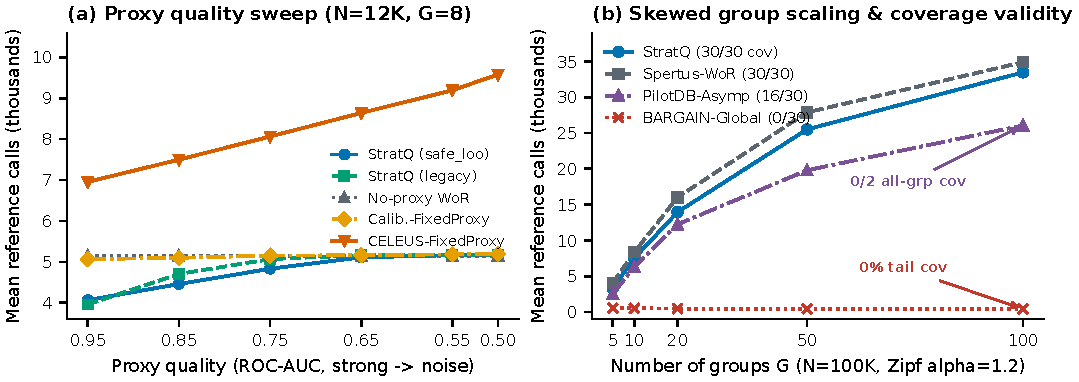
\includegraphics[width=\textwidth]{fig3_proxy_sweep_zipf.pdf}
\Description{Two-panel plot showing (a) reference calls across proxy ROC-AUC from 0.95 down to 0.50 where Safe-LOO achieves strong savings at high AUC and near-zero degradation at noise, and (b) Zipf group scaling from G=5 to G=100 showing StratQ 30/30 coverage vs PilotDB 16/30 and BARGAIN 0/30.}
\caption{(a) Proxy quality sweep ($N=12\text{K}$, $G=8$, 3 seeds): \texttt{safe\_loo} saves up to $21.1\%$ calls at AUC $0.95$, leads all comparators at moderate AUC ($0.75$--$0.85$), and stays within $+0.21\%$ of no-proxy WoR under pure noise (AUC $0.50$), whereas \texttt{CELEUS-FixedProxy} degrades to $9{,}579$ calls. (b) Skewed group scaling ($N=100\text{K}$, $\alpha=1.2$): across all 15 $(G,\alpha)$ configurations (two seeds each), \textsc{StratQ} covers all groups in $30/30$ runs, the optional-stopping CLT diagnostic in $16/30$, and the global-count surrogate's proportional group intervals in $0/30$. Coverage labels aggregate all $\alpha$ values.}
\label{fig:sweep-zipf}
\end{figure*}

\paragraph{Proxy quality sweep (AUC $0.95 \to 0.50$)}
Figure~\ref{fig:sweep-zipf}(a) isolates proxy quality on a fixed 12,000-row, 8-group Zipf snapshot ($\epsilon_g = 0.04 N_g$, 3 seeds).
At strong proxy quality (AUC $0.95$), \texttt{safe\_loo} reduces mean calls from 5,152 (\texttt{no\_proxy}) to \textbf{4,064} ($-21.1\%$), outperforming \texttt{Calibrated-FixedProxy} (5,067) and \texttt{CELEUS-FixedProxy} (6,955). The corresponding sample SDs are $32$ vs.\ $85$ calls; at AUC $0.50$, \texttt{safe\_loo} is $5{,}163\pm121$ vs.\ $5{,}152\pm85$ for no-proxy.
At moderate quality (AUC $0.85$ and $0.75$), \texttt{safe\_loo} is the single best method (4,459 and 4,832 calls), beating both \texttt{legacy} (4,704 and 5,067) and \texttt{Calibrated-FixedProxy} (5,099 and 5,152).
As the proxy degrades to near-noise and pure noise (AUC $0.55$ and $0.50$), \texttt{safe\_loo}'s LOO guard triggers fallback to $\kappa=0$, holding calls at \textbf{5,163} ($+0.21\%$ vs.\ 5,152, $3/3$ coverage).
In contrast, \texttt{CELEUS-FixedProxy} climbs monotonically to \textbf{9,579 calls} ($+85.9\%$ overhead) with $2/3$ coverage at AUC $\le 0.65$.

\paragraph{Safe-LOO ablation on Adult, SMS, and Fashion-MNIST}
Figure~\ref{fig:s1-adult}(a) and Table~\ref{tab:s1-ablation} report our matched 195-run Sprint~1 ablation (\texttt{legacy} vs.\ \texttt{safe\_loo} vs.\ \texttt{no\_proxy}, all with \texttt{safe\_rounding=True}).
On strong-proxy \textbf{Fashion-MNIST}, \texttt{safe\_loo} cuts mean calls by \textbf{$61.26\%$} (from 3,510.4 to \textbf{1,360.0}, improving even over \texttt{legacy}'s 1,411.2) while achieving the narrowest mean half-width ($3.36\%$).
On \textbf{SMS}, \texttt{safe\_loo} reduces \texttt{COUNT} calls by \textbf{$14.01\%$} (816.8 $\to$ 702.4) and remains below no-proxy on both decision queries (\texttt{HAVING}: $-1.67\%$, 863.1 $\to$ 848.7; \texttt{TOP-2}: $-0.90\%$, 865.9 $\to$ 858.1), with $10/10$ correct decisions and $10/10$ \texttt{TOP-2} certifications. It does \emph{not} beat the legacy selector: legacy uses 689.6, 835.9, and 853.2 calls on these three queries, respectively. All modes cover all groups in every run.
On weak-proxy \textbf{Adult} (with \texttt{age} and \texttt{hours} covariates), \texttt{safe\_loo} uses 4,378.0 calls vs.\ 4,337.5 for \texttt{no\_proxy} ($+0.93\%$, $30/30$ coverage), confirming that weak proxies can still incur a sub-$1\%$ gating overhead when betting steps approach the $\lambda \le 0.5$ cap.
All $195/195$ runs covered every group's true count.

\begin{figure*}[t]
\centering
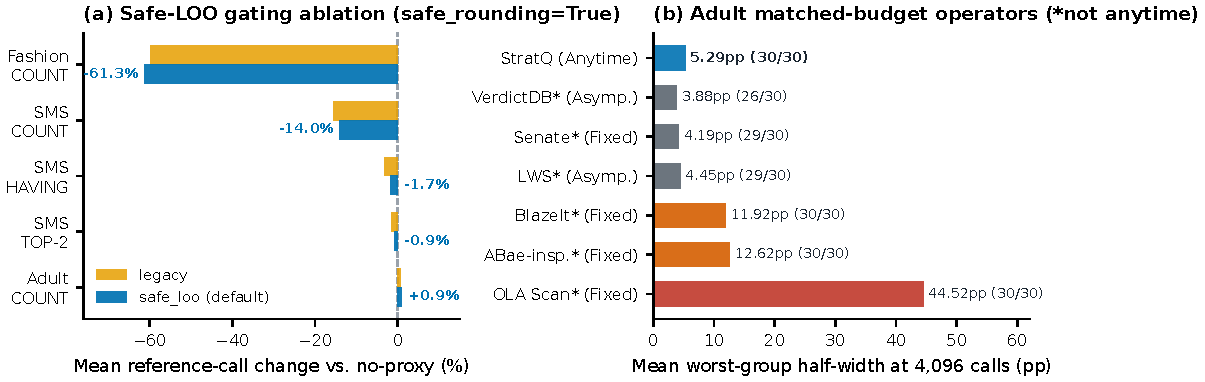
\includegraphics[width=\textwidth]{fig4_sprint1_adult.pdf}
\Description{Two-panel figure showing (a) Sprint 1 Safe-LOO vs legacy call reduction on Fashion-MNIST, SMS, and Adult, and (b) Adult 4,096-call matched-budget worst-group half-widths and simultaneous coverage across StratQ and six classical database operators.}
\caption{(a) Matched 195-run ablation (\texttt{safe\_rounding=True}): \texttt{safe\_loo} saves $61.3\%$ calls on Fashion-MNIST and $14.0\%$ on SMS \texttt{COUNT}, remains below no-proxy on SMS decisions but does not beat legacy, and limits weak-proxy Adult overhead to $+0.9\%$. (b) Adult matched-budget ($B=4{,}096$) worst-group half-width and joint coverage ($30$ seeds). Among these six fixed-look/asymptotic adaptations, only \textsc{StratQ} uses a finite-sample anytime stopping rule; the independent hypergeometric CS in the text is also anytime.}
\label{fig:s1-adult}
\end{figure*}

\begin{table}[t]
\centering
\footnotesize
\setlength{\tabcolsep}{3.5pt}
\caption{Matched 195-run Safe-LOO ablation (\texttt{safe\_rounding=True}, $\delta=0.1$). ``Max HW'' is the mean over runs of each run's largest per-group half-width. All trials achieved 100\% joint group coverage and target/decision correctness.}
\label{tab:s1-ablation}
\begin{tabular}{@{}llrrr@{}}
\toprule
Workload & Mode & Mean Calls & $\Delta$ vs.\ No-Proxy & Max HW \\
\midrule
\multirow{3}{*}{Fashion COUNT (5)}
& \texttt{no\_proxy} & 3,510.4 & 0.0\% & 3.96\% \\
& \texttt{legacy} & 1,411.2 & $-59.80\%$ & 3.84\% \\
& \textbf{\texttt{safe\_loo}} & \textbf{1,360.0} & \textbf{$-61.26\%$} & \textbf{3.59\%} \\
\midrule
\multirow{3}{*}{SMS COUNT (10)}
& \texttt{no\_proxy} & 816.8 & 0.0\% & 5.88\% \\
& \texttt{legacy} & 689.6 & $-15.57\%$ & 5.71\% \\
& \textbf{\texttt{safe\_loo}} & \textbf{702.4} & \textbf{$-14.01\%$} & \textbf{5.67\%} \\
\midrule
\multirow{3}{*}{SMS HAVING (10)}
& \texttt{no\_proxy} & 863.1 & 0.0\% & 28.11\% \\
& \texttt{legacy} & 835.9 & $-3.15\%$ & 27.43\% \\
& \textbf{\texttt{safe\_loo}} & \textbf{848.7} & \textbf{$-1.67\%$} & 29.71\% \\
\midrule
\multirow{3}{*}{SMS TOP-2 (10)}
& \texttt{no\_proxy} & 865.9 & 0.0\% & 29.18\% \\
& \texttt{legacy} & 853.2 & $-1.47\%$ & 27.43\% \\
& \textbf{\texttt{safe\_loo}} & \textbf{858.1} & \textbf{$-0.90\%$} & 29.71\% \\
\midrule
\multirow{3}{*}{Adult COUNT (30)}
& \texttt{no\_proxy} & 4,337.5 & 0.0\% & 3.97\% \\
& \texttt{legacy} & 4,369.5 & $+0.74\%$ & 3.97\% \\
& \texttt{safe\_loo} & 4,378.0 & $+0.93\%$ & 3.97\% \\
\bottomrule
\end{tabular}
\end{table}

\paragraph{High group counts and Zipf skew stress}
Figure~\ref{fig:sweep-zipf}(b) reports our 100K-row Zipf stress suite spanning $G \in \{5, 10, 20, 50, 100\}$ and $\alpha_{\text{zipf}} \in \{0.0, 0.8, 1.2\}$ (AUC $0.85$, $\epsilon_g = 0.05 N_g$, 2 seeds per cell = 30 runs per method).
\textsc{StratQ} achieves \textbf{$30/30$ ($100\%$) all-group coverage} and $100\%$ tail-group coverage across every cell, while using fewer calls than \texttt{Spertus-WoR} in \textbf{14 of 15} $(G, \alpha)$ configurations (e.g., at $G=100, \alpha=0.0$: 62,784 vs.\ 71,424 calls, saving 8,640 calls; at $G=20, \alpha=1.2$: 13,952 vs.\ 16,000; only at $G=5, \alpha=0.0$ is \textsc{StratQ} slightly higher at 3,856 vs.\ 3,664).
The global-count surrogate's proportional group intervals cover all groups in \textbf{$0/30$} runs and $0/222$ tail-group instances; the JSON does not record its global interval, so this is not a test of BARGAIN's original guarantee. The \texttt{PilotDB-Asymp} optional-stopping diagnostic covers all groups in \textbf{$16/30$ ($53.3\%$)} runs and $0/6$ at $G=100$, with pooled tail coverage $215/222=96.85\%$. Reusing a fixed-look CLT radius at data-dependent looks is a diagnostic protocol mismatch, not PilotDB's intended fixed-look use.
Optimizer overhead for \textsc{StratQ} scales cleanly from 0.32\,s ($G=5$) to 3.01\,s ($G=100, \alpha=1.2$, 33.5K calls).

\subsection{Classical Baselines, Decision Boundaries, and Routing}
\label{sec:eval-classical}

\paragraph{Six classical AQP operators on Adult}
Figure~\ref{fig:s1-adult}(b) compares \textsc{StratQ} against six published sampling/interval operators at a matched budget of $B=4{,}096$ calls on UCI Adult (30 seeds).
Only \textsc{StratQ} maintains finite-sample anytime validity across all stopping times; at 4,096 calls its mean worst-group half-width is \textbf{5.29\,pp} ($30/30$ coverage), outperforming fixed-look \textbf{BlazeIt-inspired} (11.92\,pp, $30/30$), \textbf{ABae-inspired} proxy strata (12.62\,pp, $30/30$), and unindexed \textbf{Online Aggregation} (44.52\,pp, $30/30$, where $15/30$ runs leave at least one small group completely unsampled).
Fixed-look \textbf{Senate} (4.19\,pp, $29/30$), asymptotic \textbf{LWS} (4.45\,pp, $29/30$), and asymptotic \textbf{VerdictDB} (3.88\,pp, observed $26/30$) produce narrower single-look intervals at $B=4{,}096$, illustrating the modest width price paid for finite-sample optional-stopping validity. The $26/30$ observation is not itself proof of sub-nominal population coverage.
An independent anytime grouped hypergeometric CS~\cite{wor2020} requires $4{,}581.7\pm178.8$ mean$\pm$SD calls on Adult vs.\ $4{,}337.5\pm84.8$ for no-proxy \textsc{StratQ} ($30/30$ coverage each), a 244.3-call (5.63\%) gap.

\paragraph{Decision boundaries and abstention (960 runs)}
We evaluated four 1,024-row snapshots ($G=4$, $N_g=256$) with counts $(192,128,128-d,32)$, $d\in\{0,1,16,64\}$, three budgets $\{256,768,1{,}024\}$, 20 seeds, proxy on/off, and two queries ($4\times3\times20\times2\times2=960$ trials). \textbf{All 960 runs had zero interval-coverage failures, wrong \texttt{HAVING} labels, and wrong certificates;} all 288 certified top-2 runs were correct.
At budget 256 no \texttt{HAVING} run ($\tau=128$) fully resolved. At 768 all positive-gap top-2 runs certified ($120/120$); ties abstained until census ($B=1{,}024$), where deterministic tie-breaking certified $40/40$ runs (20 seeds $\times$ two proxy settings).

\paragraph{Capped-budget routing ablation (180 matched pairs)}
Without a binding budget cap and with the proxy disabled, width-first and round-robin routing consume identical prefixes (4,337.5 mean calls across all 30 Adult seeds).
Under caps $B \in \{2{,}048, 4{,}096, 8{,}192\}$, width-first routing produces a strictly smaller worst-group half-width in \textbf{180/180 matched pairs} (e.g., at $B=4{,}096$ with proxy, mean max half-width drops from 6.67\,pp to 5.29\,pp), while the mean number of groups below 4\% falls from 5.73 to 2.40 out of nine---a direct minimax vs.\ throughput trade-off.

\paragraph{Cheap CPU live latency.}
An aligned rerun (one warm-up + ten randomized measured blocks; identical models/rows and exact batch sweep) gives Fashion-MNIST 1,430.5\,ms exact (best batch 1,024), vs.\ 577.3\,ms fresh and 423.5\,ms reused. SMS is 519.2\,ms exact (full batch), vs.\ 902.3\,ms fresh and 834.7\,ms reused, so exact batching wins. Fitting/loading are excluded. This record supersedes the older cross-study CPU timing comparison.

\subsection{Scale, Profile Amortization, and Memory Attribution}
\label{sec:eval-scale}

\begin{figure*}[t]
\centering
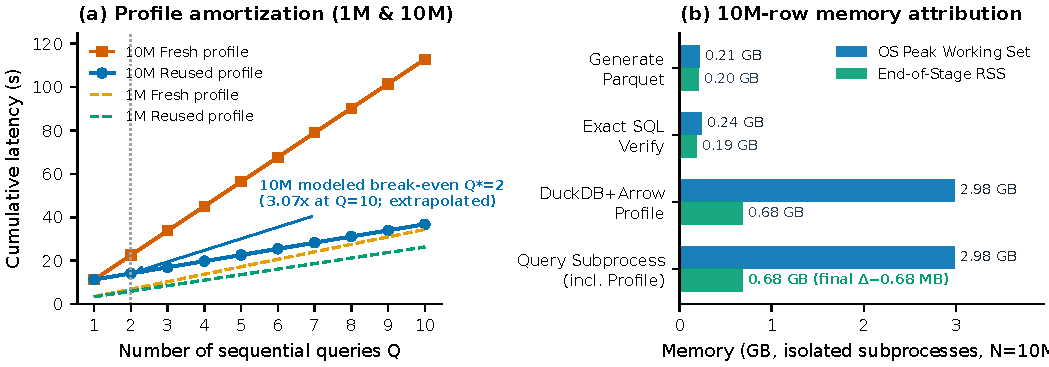
\includegraphics[width=\textwidth]{fig5_scale_memory.pdf}
\Description{Two-panel figure showing (a) cumulative latency of fresh vs reused DuckDB and Arrow profiles at 1M and 10M rows with modeled break-even at Q*=2, and (b) isolated four-stage subprocess memory breakdown at 10M rows showing profile-dominated peak working set, an 85.6 MB query traced-allocation peak, a single +21.7 MB immediate post-query RSS delta, and a -0.68 MB final post-teardown delta.}
\caption{(a) Profile amortization over sequential queries on 1M and 10M Parquet snapshots: at 10M rows, profile reuse breaks even at modeled $Q^*=2$ and achieves $3.07\times$ lower modeled cumulative latency by $Q=10$; only five queries were measured, so $Q=10$ is extrapolated. (b) Independent subprocess memory attribution at $N=10\text{M}$: DuckDB/Arrow profiling accounts for the peak working set (2.98\,GB under \texttt{tracemalloc}; 0.68\,GB end RSS). The query subprocess also rebuilds the profile, so its peak WS is not query-only. A single immediate post-query RSS delta is $+21.7$\,MB, the query-stage traced-allocation peak is 85.6\,MB, and the final post-teardown RSS delta is $-0.68$\,MB.}
\label{fig:scale-mem}
\end{figure*}

\begin{table}[t]
\centering
\footnotesize
\setlength{\tabcolsep}{3.2pt}
\caption{Isolated four-stage subprocess memory attribution at $N=10\text{M}$ rows ($G=20$, offline Boolean-label replay). ``Wall'' is subprocess-stage wall; the query stage rebuilds the profile before its 37.86\,s query-only execution. RSS deltas use the profile-end baseline and are single observations.}
\label{tab:mem-10m}
\begin{tabular}{@{}lrrrr@{}}
\toprule
Stage (Subprocess) & Wall & \texttt{tracemalloc} & Peak WS & End RSS \\
\midrule
Generate Parquet & 1.64\,s & 11.4\,MB & 0.213\,GB & 0.203\,GB \\
Exact SQL Verify & 0.06\,s & 0.0\,MB & 0.236\,GB & 0.186\,GB \\
DuckDB+Arrow Profile & 104.53\,s & 1,285.3\,MB & 2.979\,GB & 0.682\,GB \\
Query Subprocess (incl.\ Prof.) & 187.85\,s & 85.6\,MB & 2.980\,GB & 0.680\,GB \\
\quad Profile Rebuild & 103.50\,s & --- & --- & --- \\
\quad Query-only Execution & 37.86\,s & --- & --- & --- \\
\quad Immediate Post-query $\Delta$RSS & --- & --- & --- & \textbf{$+$21.69\,MB} \\
\quad Final $\Delta$RSS after Teardown & --- & --- & --- & \textbf{$-$0.68\,MB} \\
\bottomrule
\end{tabular}
\end{table}

Figure~\ref{fig:scale-mem} and Table~\ref{tab:mem-10m} evaluate $1\text{M}$ and $10\text{M}$ Parquet rows ($G=20$, offline Boolean-label replay). Without \texttt{tracemalloc}, profiling takes 0.82--0.85\,s at 1M (warm query 2.55--2.58\,s; modeled $Q^*=1$) and 8.47\,s at 10M (cold 11.28\,s, warm 2.83\,s; modeled $Q^*=2$). The 3.07$\times$ speedup at $Q=10$ extrapolates per-query medians beyond the five measured queries.
Each 10M stage ran in a separate subprocess. The query subprocess rebuilds the profile: 187.85\,s total = 103.50\,s profile + 37.86\,s query. Profiling dominates peak WS (2.979\,GB; 0.682\,GB end RSS). The query stage has an 85.6\,MB traced-allocation peak; its immediate post-query RSS delta is $+21.69$\,MB, but the final post-teardown delta is $-0.68$\,MB. These single allocator-sensitive observations are not retained-memory guarantees.
